\chapter{COMSOL Multiphysics}
\section{Introduction to COMSOL}
COMSOL Multiphysics is a commercial finite element analysis, solver, and simulation software for desktop computers designed for various disciplines in physics and engineering, namely within electrical, mechanical, fluid and chemical applications. It supports coupling phenomena, or multiphysics, where a simulation may treat multiple models or multiple physical phenomena simultaneously. Typically this involves solving coupled systems of partial differential equations. 

The main product is COMSOL Desktop, which supports a unified workflow for cross-disciplinary model building. Several add-on products are available to the software, each categorized according to application areas, namely Electrical, Structural \& Acoustics, Fluid \& Heat, Chemical, Multipurpose and Interfacing. Examples of add-on modules are the plasma module, semiconductor module, structural mechanics module, microfluids module, corrosion module, and the particle tracing module, to name a few\cite{comsol_referencemanual}. This thesis will work solely on the wave optics module, which will be introduced in the next section. The software has an integrated user-interface environment, as exemplified in figure \ref{fig:comsol_ui}, where the way of operation of the software remains the same regardless of which application module is installed. Using the built-in physics interface together with a vast support for material properties, one may build models by defining physical quantities in the geometry, such as material properties, boundary conditions, sources and fluxes, rather than defining the underlying equations. The software will internally compile a set of equations to represent the entire model. However, equation-based modeling is also supported\cite{comsol_referencemanual}.

\begin{figure}[h]
    \centering
    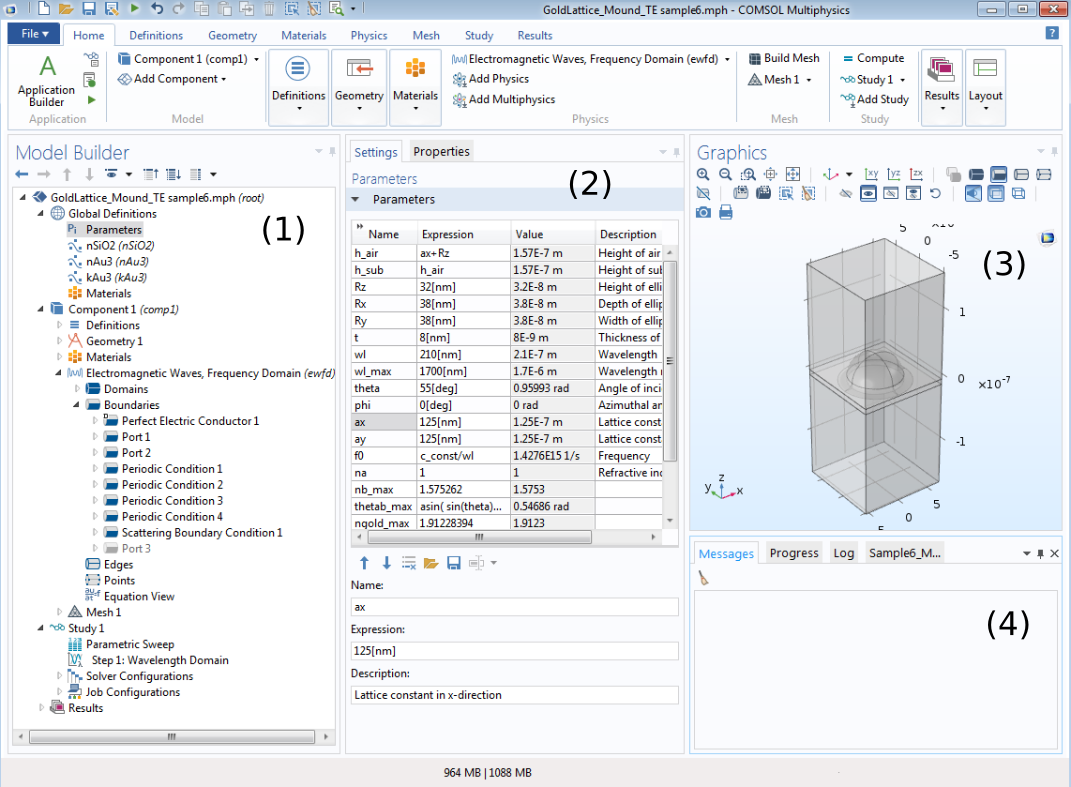
\includegraphics[width=\linewidth]{figures/Ch3/UI4.png}
    \caption{The user interface in COMSOL Desktop. (1) Model builder; overview of the model. Right-clicking a node will access context-sensitive menus. (2) Settings window; clicking a node in the model builder will display associated settings (3) Graphics window; presents interactive graphics for the Geometry, Mesh and Results nodes. (4) Information window; will display vital information during and after simulations such as solution time, simulation progress, mesh statistics and result tables.}
    \label{fig:comsol_ui}
\end{figure}

\subsection{Model builder}
\label{sec:comsol_model_builder}
A COMSOL model is controlled through the \emph{Model builder}, seen in figure \ref{fig:comsol_ui}, which essentially is a model tree containing the functionality and operations for building, solving, and displaying the results of a model. It consists of the main nodes \emph{Global Definitions} (where global parameters and materials used throughout the model are defined), \emph{Component} (the fundamental part of the model containing the model geometry with its associated physics, mesh and variables that are local to the component), \emph{Study} (where study steps are defined that form a solver configuration that computes the solution for the study) and \emph{Results} (contains tools for post-processing and analyzation of the results).

The Component node further consists of subnodes \emph{Definitions}, \emph{Geometry}, \emph{Materials}, one or several physics interfaces, and \emph{Mesh}. Some of these are explained in more detail below,
\begin{itemize}
    \item The model geometry is defined by a sequence geometric objects and operations under the Geometry node in the Model Builder. Geometries can be formed as a combination of solid objects using Boolean operations like union, intersection, and difference. Furthermore, 3D objects can be formed by defining 2D solids and then extruding or revolving these into 3D solids.
    \item In the Material node material properties are assigned to the geometric domains. The materials may be chosen from an integrated materials library, or user-specified materials defined under the Global Definitions node.
    \item The physics interface varies depending on which add-on module the user has chosen. In the example figure \ref{fig:comsol_ui}, the physics interface is \emph{Electromagnetic Waves, Frequency Domain}, which is part of the Wave Optics module.
    \item The Mesh node specifies how the geometry should be discretizied. The user may customize their own mesh or automatically generate a physics-controlled mesh based on the configurations set in the associated physics interface.
\end{itemize}

\section{The wave optics module}
The Wave Optics Module extends the functionality of COMSOL's physics interface to include dedicated tools for electromagnetic wave propagation in linear and nonlinear optical media. The module can be used to 
solve EM wave problems at optical frequencies (corresponding to wavelengths in the nm to $\mu$m region) in either frequency- or time-domain in optical structures. It supports inhomogeneous and anisotropic materials, media with gains and losses, and complex-valued material properties. 



\subsection{S-parameters}
Scattering parameters (S-parameters) are used to characterize the response in high-frequency problems.
In the Wave Optics module of COMSOL, electromagnetic waves can be excited by \emph{ports}, which is also where EM energy enters and exits the model. In 3D models, ports are fictitious planes placed on the boundaries. To convert EM field patterns on a port to a quantity describing its wave-like nature it is necessary to introduce these S-parameters. S-parameters are complex-valued, frequency dependent matrices describing the transmission and reflection of electromagnetic waves at different ports. 


S-parameters originate from transmission-line theory and are defined in terms of transmitted and reflected voltage waves. There is assumed to be no reflection directly at a port. For a model with $n$ ports, the S-parameters are \cite{comsol_waveopticsmodule}
\begin{equation}
    S = 
    \begin{pmatrix}
    S_{11} & S_{12} & \dots  & S_{1n} \\
    S_{21} & S_{22} & \dots  & S_{2n} \\
    \vdots & \vdots & \ddots & \vdots \\
    S_{n1} & S_{n2} & \dots  & S_{nn}
\end{pmatrix}
\end{equation}
where $S_{11}$ is the voltage reflection coefficient at port 1, $S_{21}$ is the voltage transmission coefficient from port 1 to port 2, and so on. The reflectance/transmittance coefficients are obtained as $\abs{S_{ij}}^2$.

\subsubsection*{S-parameter calculations}
The S-parameters are defined in terms of the electric field. Consider a model containing several ports labeled 1, 2, 3, ... and that the electric field patterns $\mathbf{E}_1$, $\mathbf{E}_2$, $\mathbf{E}_3$, ... of the fundamental modes on these ports are known. Assume that the fields are normalized with respect to the integral of the power flow across each port cross section, respectively. Port 1 is excited using the fundamental eigenmode. The computed electric field $\mathbf{E}_c$ on port 1 then consists of the excited field plus the reflected field, which can be expanded in terms of the mode fields as\cite{FEM_in_EM_jianming_jin}
\begin{equation}
    \mathbf{E}_c = \mathbf{E}_1 + \sum_{i=1}S_{i1}\mathbf{E}_i,
\end{equation}
whereas the computed field on all the other port boundaries are given by
\begin{equation}
    \mathbf{E}_c = \sum_{i=1}S_{i1}\mathbf{E}_i.
\end{equation}
Note that in this case $S_{ij}=0$ for all $j\neq1$ as there are no fields being excited on other ports than port 1. The S-parameter for mode $k$ is then given by multiplying the field delivered to port $k$ with the conjugate of field for mode $k$, and integrating over the port boundary. The first three S-parameters are given by \cite{comsol_waveopticsmodule}
\begin{subequations}
\begin{equation}
    S_{11} = \frac{\int_{\text{port} 1} (\mathbf{E}_c-\mathbf{E}_1)\cdot \mathbf{E}_1^*dA_1}{\int_{\text{port} 1} \mathbf{E}_1\cdot\mathbf{E}_1^*dA_1}
\end{equation}
\begin{equation}
    S_{21} = \frac{\int_{\text{port} 2} \mathbf{E}_c \cdot \mathbf{E}_2^*dA_2}{\int_{\text{port} 2} \mathbf{E}_2\cdot\mathbf{E}_2^*dA_2} 
\end{equation}
\begin{equation}
    S_{31} = \frac{\int_{\text{port} 3} \mathbf{E}_c \cdot \mathbf{E}_2^*dA_3}{\int_{\text{port} 3} \mathbf{E}_3\cdot\mathbf{E}_2^*dA_3} 
\end{equation}
\end{subequations}
To get $S_{22}$ and $S_{12}$ port 2 can be excited in the same way.

\subsection{The \emph{Electromagnetic Waves, Frequency Domain} interface}
The Electromagnetic Waves, Frequency Domain (EWFD) interface in COMSOL's Wave Optics module is used to solve for time-harmonic electromagnetic field distributions. The main governing equation in the interface is the time-harmonic wave equation for the electric field \text{\color{red}ref. introduser i teoridel.} The EWFD supports study types in wavelength and frequency domains (among others\cite{comsol_waveopticsmodule}), used for source driven simulations for a single wavelength/frequency or a sequence of wavelengths/frequencies.

For this physics interface, the maximum mesh element size should be limited to a fraction of the wavelength. Thus, the domain size that can be simulated scales with the wavelength and the amount of available computer memory. By default, COMSOL Multiphysics uses second-order elements\footnote{Element order refers to the type of basis function used.} to discretize the governing equations\cite{comsol_ElementOrder}, in contrast to the first-order elements illustrated in figures \ref{fig:FEM_1Ddomain} and \ref{fig:FEM_2Ddomain} with linear basis functions. As a bare minimum, two elements per wavelength are then necessary to solve the problem\footnote{The idea is fundamentally similar to the Nyquist sampling theorem in signal processing, which states that in order to recover all Fourier components of a waveform, the sampling rate must be at least twice the highest frequency of the signal.}, but such a coarse mesh would result in poor accuracy. 

In order to properly resolve the wavelength, at least five second-order elements per wavelength are typically used to resolve a wave propagating through a dielectric medium\cite{comsol_simulationToolsEM}. Local material properties should also be taken into account. In other words, a physically reliable solution requires the mesh to have a \emph{maximum element size} (\ac{mes}) no larger than
\begin{equation}
    \text{MES} \leq \frac{\lambda}{5n},
    \label{eq:MES<=lambda/5n}
\end{equation}
where $n$ is the refractive index of the given region. For discretization into first-order elements, at least 10 linear elements are required per wavelength\cite{comsol_waveopticsmodule}.

\subsubsection*{Periodic structures}
Periodic structures may be modelled by truncating the domain into a single cell with periodic conditions on selected boundaries to set up a periodicity. A typical type of periodic condition used for models involving plane waves interacting with periodic structures is \emph{Floquet periodicity}, which ensures a phase shift between the tangential components of the wave. The phase shift is determined by a wave vector and the distance between the source and destination\cite{comsol_waveopticsmodule}. 

When modelling periodic structures, \emph{periodic ports} can be used to define wave direction and polarization of the wave that enters the model. Periodic ports also compute the reflected and transmitted diffraction orders as a function of incident angles and wavelength, in addition to the fundamental mode\cite{comsol_periodicstructures}.

\cleardoublepage







